\documentclass[tikz, border=4pt]{standalone}
\usepackage{tikz}
\usetikzlibrary{quantikz2}
\begin{document}
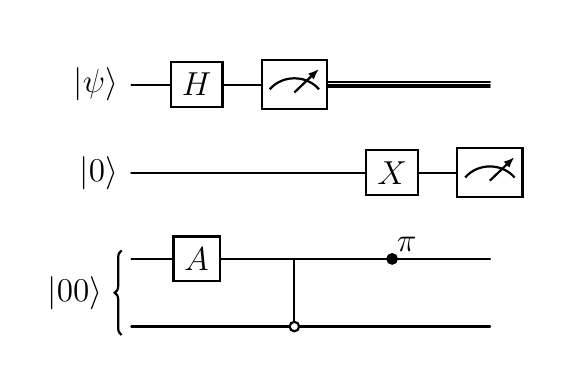
\begin{tikzpicture}[x=1cm, y=1cm]
  \node[font=\large] at (3.17,-1.93) {\pgfinterruptpicture%
  \begin{quantikz}
  \lstick{$\ket{\psi}$} & \gate{H} & \meter{} & \cw & \cw \\
  \lstick{$\ket{0}$} & \qw & \qw & \gate{X} & \meter{} \\
  \lstick[2]{$\ket{00}$} & \gate{A} & \qw & \phase{\pi} & \qw \\
   & \qw & \octrl{-1} & \qw & \qw
  \end{quantikz}%
  \endpgfinterruptpicture};
\end{tikzpicture}
\end{document}
